%%%%%%%%%%%%%%%%%%%%%%%%%%%%%%%%%%%%%%%%%
% Short Sectioned Assignment LaTeX Template Version 1.0 (5/5/12)
% This template has been downloaded from: http://www.LaTeXTemplates.com
% Original author:  Frits Wenneker (http://www.howtotex.com)
% License: CC BY-NC-SA 3.0 (http://creativecommons.org/licenses/by-nc-sa/3.0/)
%%%%%%%%%%%%%%%%%%%%%%%%%%%%%%%%%%%%%%%%%

%----------------------------------------------------------------------------------------
%	PACKAGES AND OTHER DOCUMENT CONFIGURATIONS
%----------------------------------------------------------------------------------------

\documentclass[paper=a4, fontsize=11pt]{scrartcl} % A4 paper and 11pt font size

% ---- Entrada y salida de texto -----

\usepackage[T1]{fontenc} % Use 8-bit encoding that has 256 glyphs
\usepackage[utf8]{inputenc}
%\usepackage{fourier} % Use the Adobe Utopia font for the document - comment this line to return to the LaTeX default

% ---- Idioma --------

\usepackage[spanish, es-tabla]{babel} % Selecciona el español para palabras introducidas automáticamente, p.ej. "septiembre" en la fecha y especifica que se use la palabra Tabla en vez de Cuadro

% ---- Otros paquetes ----

\usepackage{amsmath,amsfonts,amsthm} % Math packages
%\usepackage{graphics,graphicx, floatrow} %para incluir imágenes y notas en las imágenes
\usepackage{graphics,graphicx, float} %para incluir imágenes y colocarlas

% Para hacer tablas comlejas
%\usepackage{multirow}
%\usepackage{threeparttable}

%\usepackage{sectsty} % Allows customizing section commands
%\allsectionsfont{\centering \normalfont\scshape} % Make all sections centered, the default font and small caps

\usepackage{fancyhdr} % Custom headers and footers
\pagestyle{fancyplain} % Makes all pages in the document conform to the custom headers and footers
\fancyhead{} % No page header - if you want one, create it in the same way as the footers below
\fancyfoot[L]{} % Empty left footer
\fancyfoot[C]{} % Empty center footer
\fancyfoot[R]{\thepage} % Page numbering for right footer
\renewcommand{\headrulewidth}{0pt} % Remove header underlines
\renewcommand{\footrulewidth}{0pt} % Remove footer underlines
\setlength{\headheight}{13.6pt} % Customize the height of the header

\numberwithin{equation}{section} % Number equations within sections (i.e. 1.1, 1.2, 2.1, 2.2 instead of 1, 2, 3, 4)
\numberwithin{figure}{section} % Number figures within sections (i.e. 1.1, 1.2, 2.1, 2.2 instead of 1, 2, 3, 4)
\numberwithin{table}{section} % Number tables within sections (i.e. 1.1, 1.2, 2.1, 2.2 instead of 1, 2, 3, 4)

\setlength\parindent{0pt} % Removes all indentation from paragraphs - comment this line for an assignment with lots of text

\newcommand{\horrule}[1]{\rule{\linewidth}{#1}} % Create horizontal rule command with 1 argument of height

\usepackage{url}
\usepackage[pdftex]{hyperref}
\hypersetup{colorlinks,%
	citecolor=blue,%
	filecolor=blue,%
	linkcolor=black,%
	urlcolor=blue,%
	pdftex}

\graphicspath{ {images/} }

%----------------------------------------------------------------------------------------
%	TÍTULO Y DATOS DEL ALUMNO
%----------------------------------------------------------------------------------------

\title{	
\normalfont \normalsize 
\textsc{{\bf Modelos de computación (2015-2016)} \\ Grado en Ingeniería Informática \\ Universidad de Granada} \\ [25pt] % Your university, school and/or department name(s)
\horrule{0.5pt} \\[0.4cm] % Thin top horizontal rule
\huge Memoria Prácticas \\ % The assignment title
\horrule{2pt} \\[0.5cm] % Thick bottom horizontal rule
}

\author{Francisco Javier Navarro Morales} % Nombre y apellidos

\date{\normalsize\today} % Incluye la fecha actual

%----------------------------------------------------------------------------------------
% DOCUMENTO
%----------------------------------------------------------------------------------------

\begin{document}

\maketitle % Muestra el Título

\newpage %inserta un salto de página

\tableofcontents % para generar el índice de contenidos

%indice de figuras y tablas (Lo he comentado para que las referencias me salgan en orden)
%\listoffigures

%\listoftables

\newpage

%----------------------------------------------------------------------------------------
%	Cuestion 1
%----------------------------------------------------------------------------------------

\section{Practica 1: G = (V,T,P,S), donde V = {S,A,B}, T = {a,b}, el símbolo de partida es S y las reglas son:}

\begin{center}

S $\to$ aB, \qquad S $\to$ bA, \qquad A $\to$ a, \qquad A $\to$ aS, 

A $\to$ bAA, \qquad B $\to$ b, \qquad B $\to$ bS, \qquad B $\to$ aBB

\end{center}

Esta gramática genera el lenguaje: $L(G) = \{u | u \hspace{0.3em} \epsilon \hspace{0.3em} \{ a, b \}^+ \hspace{0.3em} y \hspace{0.3em} Na(u) = Nb(u) \}$, es decir, la gramática genera palabras con el mismo número de 'a' que de 'b'.
\\ \\
Podemos extraer las siguientes interpretaciones de las reglas de producción:
\begin{itemize}	
\item Interpretación de \textbf{'A'} $\to$ Genera palabras con un Símbolo Terminal 'a' de más.

\item Interpretación de \textbf{'B'} $\to$ Genera palabras con un Símbolo Terminal 'b' de más.

\item Interpretación de \textbf{'S'} $\to$ Genera una cadena con el mismo numero de 'a' que 'b'.
\end{itemize}

$\\$$ \stackrel{w = \lambda v}{\longrightarrow}$
\\

Hay que demostrar dos cosas:
\begin{itemize}	
	\item Todas las palabras generadas por la gramática tienen el mismo número de a que de b.
	
	\item Cualquier palabra con el mismo número de a que de b es generada.
\end{itemize}

$\\$ $\\$
Vamos a ir desarrollando cada posibilidad de forma que para cada paso se apliquen todas las reglas de producción posibles, inicialmente tenemos dos posibilidades:
\begin{center}
	$^{1}$S $\Rightarrow$ aB, $\qquad$ 	$^{2}$S $\Rightarrow$ bA
\end{center}

Vamos a iniciar el desarrollo para la primera:
\begin{flushleft}
\qquad S $\Rightarrow$ aB $\Rightarrow$ ab, generamos la palabra $\textbf{ab}$.\\
\qquad S $\Rightarrow$ aB $\Rightarrow$ abS $\Rightarrow$ abaB $\Rightarrow$ abab, generamos la palabra $\textbf{abab}$.\\
\qquad S $\Rightarrow$ aB $\Rightarrow$ aaBB $\Rightarrow$ aabB $\Rightarrow$ aabb, generamos la palabra $\textbf{aabb}$.\\
\end{flushleft}
Continuamos el desarrollo para la segunda posibilidad:
\begin{flushleft}
\qquad S $\Rightarrow$ bA $\Rightarrow$ ba, generamos la palabra $\textbf{ba}$.\\
\qquad S $\Rightarrow$ bA $\Rightarrow$ baS $\Rightarrow$ babA $\Rightarrow$ baba, generamos la palabra $\textbf{baba}$.\\
\qquad S $\Rightarrow$ bA $\Rightarrow$ bbAA $\Rightarrow$ bbaA $\Rightarrow$ bbaa, generamos la palabra $\textbf{bbaa}$.\\
\end{flushleft}

Hemos comprobado que podemos conseguir generar cadenas básicas con $N_{a}$(u) = $N_{b}(u)$, dónde primero hay símbolos terminales 'a' y luego 'b' ó hay símbolos terminales '(ab)$^{+}$', y lo mismo cambiando el orden de 'a' y 'b'. Si queremos generar cualquier cadena perteneciente al lenguaje lo podemos conseguir combinando las anteriores palabras generadas. Por ejemplo generemos una palabra usando todas las reglas de producción:

\begin{center}
	 S $ \stackrel{1}{\Rightarrow} $ aB 
	 $\stackrel{8}{\Rightarrow}$ aaBB 
	 $\stackrel{7}{\Rightarrow}$ aabSB 
	 $\stackrel{1}{\Rightarrow}$ aabaBB  
	 $\stackrel{8}{\Rightarrow}$  aabaaBBB 
	 $\stackrel{7}{\Rightarrow}$ aabaabSBB 
	 $\stackrel{2}{\Rightarrow}$ aabaabbABB 
	 $\stackrel{5}{\Rightarrow}$  aabaabbbAABB $\stackrel{3}{\Rightarrow}$ aabaabbbaABB $\stackrel{4}{\Rightarrow}$ aabaabbbaaSBB $\stackrel{2}{\Rightarrow}$ aabaabbbaabABB $\stackrel{3}{\Rightarrow}$ aabaabbbaabaBB $\stackrel{6}{\Rightarrow}$ aabaabbbaababB $\stackrel{6}{\Rightarrow}$ aabaabbbaababb
\end{center}

Podemos apreciar que encima de cada fecha indicamos el número de la regla utilizada (las identificamos contando de izquierda a derecha y de arriba hacia abajo) en este ejemplo hemos usado las 8 reglas de producción que nos brinda la gramática, comprobando que la palabra que genera \textbf{'aabaabbbaababb'} contiene el mismo número de símbolos terminales 'a' que 'b', en concreto N = 7. Con este ejemplo demostramos también que combinando las reglas de producción podemos generar cualquier palabra con la peculiaridad de que el número de 'a' coincide con el de 'b'.

%----------------------------------------------------------------------------------------
%	Cuestion 2
%----------------------------------------------------------------------------------------

\section{Practica 2: Determinar si la gramática G = (\{S, A, B\}, \{a, b, c, d\}, P, S) genera un lenguaje de tipo 3 donde P es el conjunto de reglas de producción:}
\begin{center}
$
S \rightarrow AB, \qquad A \rightarrow Ab, \qquad A \rightarrow a, 
$
$
\qquad B \rightarrow cB, \qquad B \rightarrow d
$
\end{center}


\textbf{Gramática libre del contexto, es decir, de tipo 2}: Los símbolos terminales dependen entre ellos y alguna regla de producción es del tipo: $A \rightarrow u$ ; $A \rightarrow U$.

Esta \textbf{gramática genera el lenguaje $L(G) = \{a b^{i} c^{j} d : i, j \hspace{0.3em} \epsilon \hspace{0.3em} \mathbb{N} \}$} 
\\ \\
Primero, vamos a \textbf{demostrar que a partir de las reglas de producción de tipo 2 se genera el lenguaje L(G)}.
\\ \\
Comenzamos con el símbolo de partida ''S'':
\\ \\
$
S \rightarrow \underline{A}B^{1} \rightarrow \underline{A}bB^{2} \rightarrow \underline{A}bbB^{2} \rightarrow ab^{i}\underline{B}^{3} \rightarrow ab^{i}c\underline{B}^{4} \rightarrow ab^{i}cc\underline{B}^{4} \rightarrow ab^{i}c^{j}\underline{B}^{4} \rightarrow ab^{i}c^{j}d^{5}
$
\\ \\
\\ \\

Notas sup-indices:
\\
1. Como el lenguaje L(G) comienza por un símbolo terminal ''a'' seguidos por i veces el símbolo terminal ''b'', aplicamos la regla de producción $A \rightarrow Ab$, ya que a partir de la variable ''A'' podemos generar i veces el símbolo terminal ''b'' y generar el símbolo terminal ''a'' de la primera posición cuando se desee.
\\
2. Para generar el símbolo terminal ''b'' i veces producimos la regla de producción $A \rightarrow Ab$ y generamos $b^{i}$ veces el símbolo terminal ''b''.
\\
3. Como el lenguaje L(G) comienza por el símbolo terminal ''a'' y ya disponemos del símbolo terminal $b^{i}$, aplicamos la regla de producción $A \rightarrow a$ para obtener el primer símbolo terminal del lenguaje L(G).
\\
4. El lenguaje L(G) dispone de j veces el símbolo terminal ''c'' para ello vamos aplicando la regla de producción $B \rightarrow cB$ sobre la variable ''B'' para generar los $c^{j}$ símbolos terminales.
\\
5. El lenguaje L(G) termina con el símbolo terminal ''d'', por tanto, aplicamos la regla de producción $B \rightarrow d$ sobre la variable ''B'' para obtener el símbolo terminal ''d''.
\\ \\
Como podemos observar con las reglas de producción de tipo 2, el lenguaje L(G) se puede generar y como patrón podemos sacar que para obtener los $b^{i}$ símbolos terminales vamos aplicando la regla de producción sobre la variable ''A'' y para obtener los símbolos terminales $c^{j}$ aplicamos la regla de producción sobre la variable ''B''.
\\ \\
Segundo, para \textbf{generar un lenguaje de tipo 3 (Regular)}: Los símbolos terminales no dependen entre ellos y las reglas de producción tienen que ser del tipo 3, ya que si las reglas de producción son del tipo 3 el lenguaje generado es de tipo 3.
\\ \\
Las reglas de producción de tipo 3 contienen 1 solo símbolo terminal a la izquierda o son del tipo: $A \rightarrow uB$ ; $A \rightarrow u$ ; $A \rightarrow B$.
\\ \\
Por tanto, para generar el lenguaje de tipo 3 debemos crear las siguientes reglas de producción de tipo 3:
\begin{itemize}
	\item $S \rightarrow aB$ : Como símbolo de partida comenzamos con la variable ''S'', por tanto en el primer paso producimos el símbolo terminal ''a'' primero que se necesita y con la variable ''B'' vamos obteniendo los $b^{i}$ símbolos terminales.
	\item $B \rightarrow bB$ : Con la variable ''B'' obtenemos los $b^{i}$ símbolos terminales.
	\item $B \rightarrow C$ : Una vez obtenidos los $b^{i}$ símbolos terminales deseados para obtener los $c^{j}$ símbolos terminales, producimos un cambio de variable para generar la producción de los símbolos terminales ''c''. 
	\item $C \rightarrow cC$ : Con la variable ''C'' generamos la producción de los $c^{j}$ símbolos terminales deseados.
	\item $C \rightarrow d$ : Para acabar con la generación del lenguaje necesitamos generar a partir de la variable ''C'' un símbolo terminal ''d''.
\end{itemize}
Por tanto, con estas reglas de producción de tipo 3 generamos una gramática de tipo 3, tal y como indica el lenguaje L(G).

%----------------------------------------------------------------------------------------
%	Cuestion 3
%----------------------------------------------------------------------------------------
\section{Practica 3: Diseñar un autómata finito determinístico que acepte cadenas que contienen las subcadenas '0110' y '1000'. Las subcadenas pueden aparecer juntas o separadas, también pueden contener más símbolos (0+1) delante o detras de ellas.}

Para comenzar esta práctica lo más sencillo es\textbf{ diseñar el autómata no determinístico} que acepta las cadenas que nos pide el ejercicio. Nos ayudamos de los ejemplos de los autómatas que son capaces de reconocer palaras que contienen las subcadenas '0110' ó '1000, de esta forma conseguimos diseñar el autómata que necesitamos de forma muy fácil, para ello \textbf{seguimos los siguientes pasos}:

\begin{itemize}
	\item Q4 deja de ser un nodo final y P0 deja de ser un nodo inicial.
	\item Unimos los dos autómatas añadiendo una transición nula entre Q4 y P0.
	
\end{itemize}

\begin{figure}[H]
	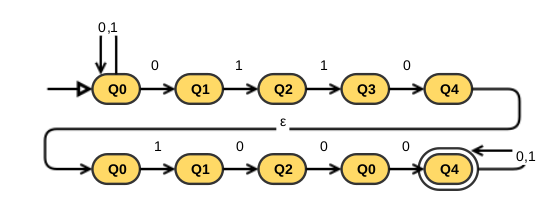
\includegraphics[scale=0.8]{prac3A.png}
	\caption{NonDeterministic finite automaton(NFA)}
\end{figure}

Los autómatas no determinísticos son muy ineficientes porque exploran todas las posibilidades. Para resolver el problema que tenemos entre las manos de una forma más eficiente vamos a tranformarlo en un autómata que para cada símbolo leido sepa que acción debe realizar. Es un proceso exponencial a medida en que crece el número de nodos en el 'NFA', para no equivocarnos vamos a realizar una tabla donde indiquemos para cada nodo cual es la acción que realiza al leer cierto símbolo de la cinta de entrada.

\begin{table}[H]
	\begin{center}
			\begin{tabular}{|c|c|c|c|c|c|}
			\hline
			\textbf{Símbolo} & \textbf{Q0} & \textbf{Q1} & \textbf{Q2} & \textbf{Q3} & \textbf{Q4} \\
			\hline \hline
			0 & \{Q0,Q1\} & \{Ø\} & \{Ø\} & \{Q4,P0\} & \{Q4,P0\}\\ \hline
			1 & \{Q0\} & \{Q2\} & \{Q3\} & \{Ø\} & \{Q4,P0,P1\} \\ \hline
		\end{tabular}
	\end{center}
		\caption{Tabla nodos Q.}
		\label{tabla:nodosQ}
\end{table}  

\begin{table}[H]
	\begin{center}
		\begin{tabular}{|c|c|c|c|c|c|}
			\hline
			\textbf{Símbolo} & \textbf{P0} & \textbf{P1} & \textbf{P2} & \textbf{P3} & \textbf{P4} \\
			\hline \hline
			0 & \{P0\} & \{P2\} & \{P3\} & \{P4\} & \{P4\}\\ \hline
			1 & \{P0,P1\} & \{Ø\} & \{Ø\} & \{Ø\} & \{P4\} \\ \hline
		\end{tabular}
	\end{center}
	\caption{Tabla nodos P.}
	\label{tabla:nodosP}
\end{table} 

Para construir nuestro autómata determinístico nos apoyaremos de las tablas que hemos creado. \textbf{Comprobamos para cada estado} de los que tenemos entre \textbf{\{<estados>\}} a que \textbf{estado(s) pasa} según lea un 0/1, si tenemos un \textbf{estado compuesto} por 2 o más estados tenemos que realizar el proceso para cada subestado y el \textbf{resultado será la unión} de los resultados de cada subestado. Una vez generado el nuevo estado tenemos \textbf{dos posibilidades} que el \textbf{nuevo estado se repita}, en este caso trazamos una flecha desde el estado actual hasta el estado obtenido(etiquetando dicha flecha con el símbolo que produce el cambio de estados); por otra parte, si \textbf{es un nuevo estado} debemos colocarlo unidos por una flecha etiquetada. \textbf{Repetimos} todo el proceso hasta que todos los estados tengan un estado objetivo para cada símbolo posible(en nuestro caso 0/1).

\begin{figure}[H]
	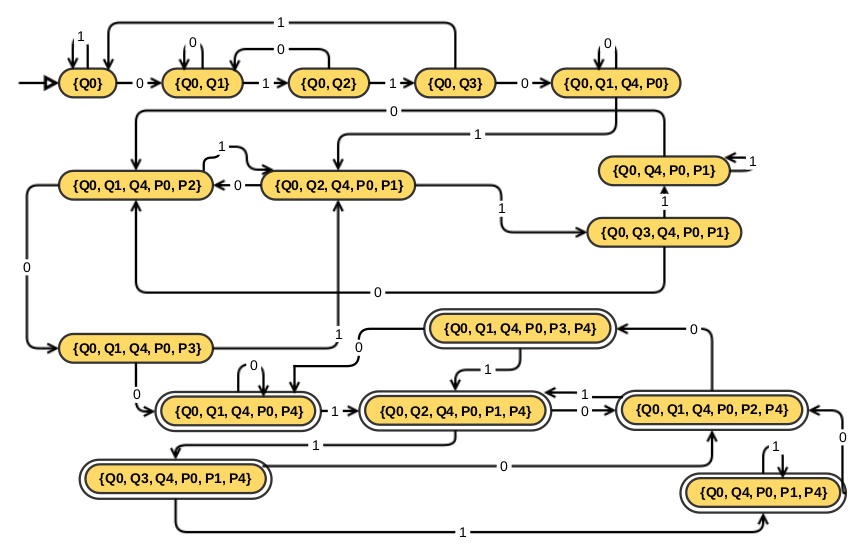
\includegraphics[scale=0.55]{prac3.png}
	\caption{Deterministic finite automaton(DFA)}
\end{figure}



%Referencias - Con ambas etiquetas se llama al fichero citas.bib
%\bibliography{citas} %archivo citas.bib que contiene las entradas 
%\bibliographystyle{ieeetr} % hay varias formas de citar

\end{document}